\documentclass[twoside]{book}

% Packages required by doxygen
\usepackage{fixltx2e}
\usepackage{calc}
\usepackage{doxygen}
\usepackage[export]{adjustbox} % also loads graphicx
\usepackage{graphicx}
\usepackage[utf8]{inputenc}
\usepackage{makeidx}
\usepackage{multicol}
\usepackage{multirow}
\PassOptionsToPackage{warn}{textcomp}
\usepackage{textcomp}
\usepackage[nointegrals]{wasysym}
\usepackage[table]{xcolor}

% Font selection
\usepackage[T1]{fontenc}
\usepackage[scaled=.90]{helvet}
\usepackage{courier}
\usepackage{amssymb}
\usepackage{sectsty}
\renewcommand{\familydefault}{\sfdefault}
\allsectionsfont{%
  \fontseries{bc}\selectfont%
  \color{darkgray}%
}
\renewcommand{\DoxyLabelFont}{%
  \fontseries{bc}\selectfont%
  \color{darkgray}%
}
\newcommand{\+}{\discretionary{\mbox{\scriptsize$\hookleftarrow$}}{}{}}

% Page & text layout
\usepackage{geometry}
\geometry{%
  a4paper,%
  top=2.5cm,%
  bottom=2.5cm,%
  left=2.5cm,%
  right=2.5cm%
}
\tolerance=750
\hfuzz=15pt
\hbadness=750
\setlength{\emergencystretch}{15pt}
\setlength{\parindent}{0cm}
\setlength{\parskip}{3ex plus 2ex minus 2ex}
\makeatletter
\renewcommand{\paragraph}{%
  \@startsection{paragraph}{4}{0ex}{-1.0ex}{1.0ex}{%
    \normalfont\normalsize\bfseries\SS@parafont%
  }%
}
\renewcommand{\subparagraph}{%
  \@startsection{subparagraph}{5}{0ex}{-1.0ex}{1.0ex}{%
    \normalfont\normalsize\bfseries\SS@subparafont%
  }%
}
\makeatother

% Headers & footers
\usepackage{fancyhdr}
\pagestyle{fancyplain}
\fancyhead[LE]{\fancyplain{}{\bfseries\thepage}}
\fancyhead[CE]{\fancyplain{}{}}
\fancyhead[RE]{\fancyplain{}{\bfseries\leftmark}}
\fancyhead[LO]{\fancyplain{}{\bfseries\rightmark}}
\fancyhead[CO]{\fancyplain{}{}}
\fancyhead[RO]{\fancyplain{}{\bfseries\thepage}}
\fancyfoot[LE]{\fancyplain{}{}}
\fancyfoot[CE]{\fancyplain{}{}}
\fancyfoot[RE]{\fancyplain{}{\bfseries\scriptsize Generated by Doxygen }}
\fancyfoot[LO]{\fancyplain{}{\bfseries\scriptsize Generated by Doxygen }}
\fancyfoot[CO]{\fancyplain{}{}}
\fancyfoot[RO]{\fancyplain{}{}}
\renewcommand{\footrulewidth}{0.4pt}
\renewcommand{\chaptermark}[1]{%
  \markboth{#1}{}%
}
\renewcommand{\sectionmark}[1]{%
  \markright{\thesection\ #1}%
}

% Indices & bibliography
\usepackage{natbib}
\usepackage[titles]{tocloft}
\setcounter{tocdepth}{3}
\setcounter{secnumdepth}{5}
\makeindex

% Hyperlinks (required, but should be loaded last)
\usepackage{ifpdf}
\ifpdf
  \usepackage[pdftex,pagebackref=true]{hyperref}
\else
  \usepackage[ps2pdf,pagebackref=true]{hyperref}
\fi
\hypersetup{%
  colorlinks=true,%
  linkcolor=blue,%
  citecolor=blue,%
  unicode%
}

% Custom commands
\newcommand{\clearemptydoublepage}{%
  \newpage{\pagestyle{empty}\cleardoublepage}%
}

\usepackage{caption}
\captionsetup{labelsep=space,justification=centering,font={bf},singlelinecheck=off,skip=4pt,position=top}

%===== C O N T E N T S =====

\begin{document}

% Titlepage & ToC
\hypersetup{pageanchor=false,
             bookmarksnumbered=true,
             pdfencoding=unicode
            }
\pagenumbering{roman}
\begin{titlepage}
\vspace*{7cm}
\begin{center}%
{\Large My Project }\\
\vspace*{1cm}
{\large Generated by Doxygen 1.8.11}\\
\end{center}
\end{titlepage}
\clearemptydoublepage
\tableofcontents
\clearemptydoublepage
\pagenumbering{arabic}
\hypersetup{pageanchor=true}

%--- Begin generated contents ---
\chapter{File Index}
\section{File List}
Here is a list of all files with brief descriptions\+:\begin{DoxyCompactList}
\item\contentsline{section}{\hyperlink{Lab1_8c}{Lab1.\+c} }{\pageref{Lab1_8c}}{}
\end{DoxyCompactList}

\chapter{File Documentation}
\hypertarget{UserDefinedLiteral_8cpp}{}\section{User\+Defined\+Literal.\+cpp File Reference}
\label{UserDefinedLiteral_8cpp}\index{User\+Defined\+Literal.\+cpp@{User\+Defined\+Literal.\+cpp}}
{\ttfamily \#include $<$iostream$>$}\\*
Include dependency graph for User\+Defined\+Literal.\+cpp\+:
\nopagebreak
\begin{figure}[H]
\begin{center}
\leavevmode
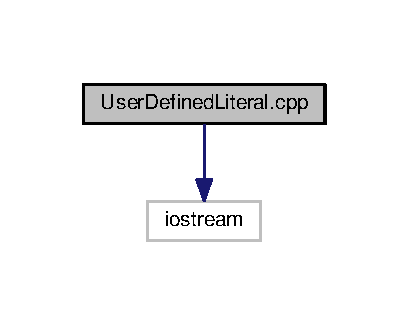
\includegraphics[width=196pt]{UserDefinedLiteral_8cpp__incl}
\end{center}
\end{figure}
\subsection*{Functions}
\begin{DoxyCompactItemize}
\item 
long double \hyperlink{UserDefinedLiteral_8cpp_a90daec3c9a9225f5660cb6406617e813}{operator\char`\"{}\char`\"{}\+\_\+kg} (long double x)
\item 
long double \hyperlink{UserDefinedLiteral_8cpp_a85bd9a0116e836b0afe077231e9b9ac5}{operator\char`\"{}\char`\"{}\+\_\+g} (long double x)
\item 
long double \hyperlink{UserDefinedLiteral_8cpp_a42788678edb94f3275a3501ef7a00de2}{operator\char`\"{}\char`\"{}\+\_\+mg} (long double x)
\item 
int \hyperlink{UserDefinedLiteral_8cpp_ae66f6b31b5ad750f1fe042a706a4e3d4}{main} ()
\end{DoxyCompactItemize}


\subsection{Function Documentation}
\index{User\+Defined\+Literal.\+cpp@{User\+Defined\+Literal.\+cpp}!main@{main}}
\index{main@{main}!User\+Defined\+Literal.\+cpp@{User\+Defined\+Literal.\+cpp}}
\subsubsection[{\texorpdfstring{main()}{main()}}]{\setlength{\rightskip}{0pt plus 5cm}int main (
\begin{DoxyParamCaption}
{}
\end{DoxyParamCaption}
)}\hypertarget{UserDefinedLiteral_8cpp_ae66f6b31b5ad750f1fe042a706a4e3d4}{}\label{UserDefinedLiteral_8cpp_ae66f6b31b5ad750f1fe042a706a4e3d4}

\begin{DoxyCode}
28 \{
29     \textcolor{keywordtype}{long} \textcolor{keywordtype}{double} weight = 3.6\_kg;
30     cout << weight << endl;
31     cout << ( weight + 2.3\_mg ) << endl;
32     cout << ( 32.3\_kg / 2.0\_g ) << endl;
33     cout << ( 32.3\_mg *2.0\_g ) << endl;
34     \textcolor{keywordflow}{return} 0;
35 \}\end{DoxyCode}
\index{User\+Defined\+Literal.\+cpp@{User\+Defined\+Literal.\+cpp}!operator\char`\"{}\char`\"{}\+\_\+g@{operator""""\+\_\+g}}
\index{operator\char`\"{}\char`\"{}\+\_\+g@{operator""""\+\_\+g}!User\+Defined\+Literal.\+cpp@{User\+Defined\+Literal.\+cpp}}
\subsubsection[{\texorpdfstring{operator""""\+\_\+g(long double x)}{operator""_g(long double x)}}]{\setlength{\rightskip}{0pt plus 5cm}long double operator\char`\"{}\char`\"{}\+\_\+g (
\begin{DoxyParamCaption}
\item[{long double}]{x}
\end{DoxyParamCaption}
)}\hypertarget{UserDefinedLiteral_8cpp_a85bd9a0116e836b0afe077231e9b9ac5}{}\label{UserDefinedLiteral_8cpp_a85bd9a0116e836b0afe077231e9b9ac5}

\begin{DoxyCode}
16 \{
17     \textcolor{keywordflow}{return} x;
18 \}
\end{DoxyCode}
\index{User\+Defined\+Literal.\+cpp@{User\+Defined\+Literal.\+cpp}!operator\char`\"{}\char`\"{}\+\_\+kg@{operator""""\+\_\+kg}}
\index{operator\char`\"{}\char`\"{}\+\_\+kg@{operator""""\+\_\+kg}!User\+Defined\+Literal.\+cpp@{User\+Defined\+Literal.\+cpp}}
\subsubsection[{\texorpdfstring{operator""""\+\_\+kg(long double x)}{operator""_kg(long double x)}}]{\setlength{\rightskip}{0pt plus 5cm}long double operator\char`\"{}\char`\"{}\+\_\+kg (
\begin{DoxyParamCaption}
\item[{long double}]{x}
\end{DoxyParamCaption}
)}\hypertarget{UserDefinedLiteral_8cpp_a90daec3c9a9225f5660cb6406617e813}{}\label{UserDefinedLiteral_8cpp_a90daec3c9a9225f5660cb6406617e813}

\begin{DoxyCode}
10 \{
11     \textcolor{keywordflow}{return} x*1000;
12 \}
\end{DoxyCode}
\index{User\+Defined\+Literal.\+cpp@{User\+Defined\+Literal.\+cpp}!operator\char`\"{}\char`\"{}\+\_\+mg@{operator""""\+\_\+mg}}
\index{operator\char`\"{}\char`\"{}\+\_\+mg@{operator""""\+\_\+mg}!User\+Defined\+Literal.\+cpp@{User\+Defined\+Literal.\+cpp}}
\subsubsection[{\texorpdfstring{operator""""\+\_\+mg(long double x)}{operator""_mg(long double x)}}]{\setlength{\rightskip}{0pt plus 5cm}long double operator\char`\"{}\char`\"{}\+\_\+mg (
\begin{DoxyParamCaption}
\item[{long double}]{x}
\end{DoxyParamCaption}
)}\hypertarget{UserDefinedLiteral_8cpp_a42788678edb94f3275a3501ef7a00de2}{}\label{UserDefinedLiteral_8cpp_a42788678edb94f3275a3501ef7a00de2}

\begin{DoxyCode}
22 \{
23     \textcolor{keywordflow}{return} x / 1000;
24 \}
\end{DoxyCode}

%--- End generated contents ---

% Index
\backmatter
\newpage
\phantomsection
\clearemptydoublepage
\addcontentsline{toc}{chapter}{Index}
\printindex

\end{document}
